\documentclass[11pt,a4paper]{ctexart}

\usepackage[margin=2.6cm]{geometry}
\usepackage{amsmath,amssymb,amsthm}
\usepackage{graphicx}
\usepackage{booktabs}
\usepackage{hyperref}
\usepackage{xcolor}
\usepackage{listings}
\usepackage{caption}

\graphicspath{{figures/}}
\hypersetup{colorlinks=true, linkcolor=blue!50!black, urlcolor=blue!60!black}
\lstset{
  basicstyle=\ttfamily\small,
  breaklines=true,
  frame=single,
  columns=fullflexible,
  backgroundcolor=\color{gray!7}
}

\newtheorem{definition}{定义}[section]
\newtheorem{theorem}{定理}[section]
\newtheorem{lemma}{引理}[section]
\newtheorem{proposition}{命题}[section]
\newtheorem{example}{例}[section]

\title{第 15 章 \quad Residual Bootstrap / 残差 Bootstrap}
\author{基于 \textit{A Course in Time Series Analysis} 的中文讲义与 Python 实践}
\date{}

\begin{document}
\maketitle

\section*{本章学习目标}

本章按照原文 \textit{Residual Bootstrap for estimation in autoregressive processes} 的小节顺序整理，保留主要定义、定理、模型公式和练习方向，并将原文中的 R 实践思路改写为 Python 工程实践。

完成本章后，应能够：
\begin{itemize}
  \item 理解 AR 模型残差 Bootstrap 的算法步骤；
  \item 区分真实残差、中心化残差和 bootstrap 残差；
  \item 理解 bootstrap 估计量抽样性质；
  \item 掌握 Wasserstein/分布距离在证明中的作用；
  \item 说明何时 residual bootstrap 能近似参数估计分布。
\end{itemize}

\section{残差 Bootstrap}

对 AR(p)
\[
  X_t=\phi_1X_{t-1}+\cdots+\phi_pX_{t-p}+\varepsilon_t,
\]
先估计 \(\hat\phi\)，得到残差
\[
  \hat\varepsilon_t=X_t-\hat\phi_1X_{t-1}-\cdots-\hat\phi_pX_{t-p}.
\]
中心化后从 \(\{\hat\varepsilon_t-\bar{\hat\varepsilon}\}\) 中有放回抽样，得到 bootstrap 创新 \(\varepsilon_t^+\)，再递推生成
\[
  X_t^+=\hat\phi_1X_{t-1}^++\cdots+\hat\phi_pX_{t-p}^+ + \varepsilon_t^+.
\]
对 bootstrap 样本重新估计参数，重复多次即可近似 \(\hat\phi\) 的抽样分布。

\section{残差 Bootstrap 的抽样性质}

原文通过若干引理证明 bootstrap 残差分布接近真实创新分布，并进一步证明 bootstrap 估计量能近似原估计量的分布。

\begin{lemma}[分布距离，原文 Lemma 15.2.1]
两个概率测度在适当距离 \(d(\alpha,\beta)\) 下收敛，可等价刻画相应随机变量分布的弱收敛。
\end{lemma}

\begin{lemma}[bootstrap 残差，原文 Lemma 15.2.2]
在 AR 参数估计相合和残差中心化条件下，bootstrap 残差的经验分布逼近真实创新分布。
\end{lemma}

\begin{lemma}[bootstrap 序列近似，原文 Lemma 15.2.3--15.2.4]
由 bootstrap 创新递推生成的序列，其样本矩阵和协方差项可逼近理论对应量，从而支持 bootstrap 参数估计的渐近有效性。
\end{lemma}

\section{算法总结}

残差 Bootstrap 的实务步骤为：
\begin{enumerate}
  \item 拟合 AR(p) 并保存参数 \(\hat\phi\)；
  \item 计算并中心化残差；
  \item 重抽样残差生成 \(\varepsilon_t^+\)；
  \item 使用 \(\hat\phi\) 和 \(\varepsilon_t^+\) 递推生成 \(X_t^+\)；
  \item 对 \(X_t^+\) 重新估计，得到 \(\hat\phi^+\)；
  \item 用 \(\hat\phi^+-\hat\phi\) 的经验分布构造标准误、置信区间或分位数。
\end{enumerate}

该方法依赖 AR 模型设定合理、残差近似独立同分布和参数估计稳定。

\section{原文逐段补充与证明细节}

本章开头先回顾前文的渐近抽样理论。前面已经研究过若干估计量的渐近分布，例如自回归参数的最小二乘估计量，以及用于估计 ARMA 参数的高斯最大似然估计量。这些渐近分布可以用于统计检验和置信区间构造。然而，渐近结果只在样本量相对较大时近似有效；当样本量较小时，正态近似可能并不可靠，需要更好的有限样本近似。

即使愿意使用渐近分布，也常常需要估计方差或偏差。有时这些表达式难以推导，或者推导成本很高。Bootstrap 的作用正在于此：它通过从样本本身构造近似分布，来估计估计量的方差、偏差、置信区间等性质。原文引用 Wikipedia 的说法：Bootstrap 是通过从近似分布中抽样，并在这些抽样上测量估计量性质，从而估计估计量性质的一种实践。直观地说，Bootstrap 是“从样本中再抽样”。每一个重抽样样本都被当作来自总体的新样本；利用这些“新的”多个实现，可以近似参数估计量的置信区间和方差。

必须注意，现实中我们并没有真的得到多个独立样本。重复重抽样并不会凭空创造新信息；它只是利用现有样本构造一个近似总体。因此，重抽样次数越多并不等于信息越多，但它能帮助我们理解估计量的有限样本分布。本章将详细说明残差 bootstrap 方法，并证明在渐近意义下，bootstrap 分布与估计量的渐近分布一致。

残差 bootstrap 最早由 J. P. Kreiss 提出，Kreiss (1997) 是一篇很好的综述。Franke and Kreiss (1992) 还给出了对 \(AR(\infty)\) 过程的扩展。早期关于 bootstrap 理论的重要论文包括 Bickel and Freedman (1981)。时间序列中还有其他 bootstrap 方法，例如周期图 bootstrap、block bootstrap、Kalman filter bootstrap 等。这些方法不仅用于估计方差，也可用于确定模型阶数等问题。频域方法可参考 Dahlhaus and Janas (1996) 和 Franke and Härdle (1992)，子抽样方法综述可参考 Politis 等人的工作。

\subsection{残差 bootstrap 的模型假设}

原文设定时间序列 \(\{X_t\}\) 满足平稳、因果的 AR(p) 过程：
\[
  X_t=\sum_{j=1}^p\phi_jX_{t-j}+\varepsilon_t,
\]
其中 \(\{\varepsilon_t\}\) 为 iid 随机变量，均值为 0，方差为 1。AR 特征多项式的根的绝对值都大于 \(1+\delta\)，这意味着过程不仅稳定，而且根与单位圆有正距离。为简化讨论，原文假定阶数 \(p\) 已知。

定义滞后向量
\[
  X_{t-1}'=(X_{t-1},\ldots,X_{t-p}).
\]
第一步构造样本矩阵和样本向量：
\[
  \hat\Gamma_p=\frac1n\sum_{t=p+1}^nX_{t-1}X_{t-1}',
  \qquad
  \hat\gamma_p=\frac1n\sum_{t=p+1}^nX_{t-1}X_t.
  \tag{15.1}
\]
于是自回归参数估计量写作
\[
  \hat\phi_n=(\hat\phi_1,\ldots,\hat\phi_p)'
  =\hat\Gamma_p^{-1}\hat\gamma_p.
\]
这正是条件最小二乘或 Yule-Walker 型回归估计的矩阵写法。

第二步估计残差：
\[
  \hat\varepsilon_t=X_t-\sum_{j=1}^p\hat\phi_jX_{t-j}.
\]
第三步用这些估计残差构造经验分布函数：
\[
  \hat F_n(x)
  =\frac1{n-p}\sum_{t=p+1}^n I_{(-\infty,\hat\varepsilon_t]}(x).
\]
从 \(\hat F_n\) 抽样等价于：以概率 \((n-p)^{-1}\) 从每一个估计残差 \(\hat\varepsilon_t\) 中抽取一个值。

第四步，从 \(\hat F_n\) 独立抽取 \(n\) 个 bootstrap 创新，记为 \(\{\varepsilon_k^+\}\)。第五步，给定初始值 \(X_k^+=\varepsilon_k^+\)（\(1\le k\le p\)），对 \(k>p\) 用
\[
  X_k^+=\sum_{j=1}^p\hat\phi_jX_{k-j}^+ + \varepsilon_k^+
\]
递推生成 bootstrap 序列。第六步，重复该过程 \(N\) 次，得到 \(N\) 个 bootstrap 样本。第七步，对每个 bootstrap 样本重新计算 \(\Gamma_p^+\)、\(\gamma_p^+\) 和
\[
  \hat\phi_n^+=(\Gamma_p^+)^{-1}\gamma_p^+.
\]
第八步，用这些 \(\hat\phi_n^+\) 的经验分布估计 \(\hat\phi_n-\phi\) 的分布，或者估计 \(\hat\phi_n\) 的方差。

\subsection{bootstrap 抽样性质的目标}

第 15.2 节要证明：
\[
  \sqrt n(\hat\phi_n^+-\hat\phi_n)
\]
的分布与
\[
  \sqrt n(\hat\phi_n-\phi)
\]
的分布渐近一致。这说明在大样本极限下，使用 bootstrap 分布不会比使用渐近正态近似更差。原文同时提醒：这个结论并不自动说明 bootstrap 分布对有限样本分布的近似一定优于普通正态近似。若要比较更高阶精度，需要使用 Edgeworth 展开等工具。

为了证明两个分布渐近一致，原文使用如下距离。对 \(p>1\)，定义
\[
  d_p(H,G)=\inf_{X\sim H,Y\sim G}\{E|X-Y|^p\}^{1/p}.
\]
这里下确界取遍所有边际分布分别为 \(H\) 和 \(G\) 的联合分布。当 \(p=2\) 时，该距离称为 Mallows 距离：
\[
  d_2(H,G)=\inf_{X\sim H,Y\sim G}\{E|X-Y|^2\}^{1/2}.
\]
如果 \(H=G\)，可取 \(X=Y\)，于是距离为 0。为了简化记号，原文把随机变量的边际分布记入符号中，写作 \(d_p(X,Y)\)。该距离满足三角不等式。

\begin{lemma}[Mallows 距离与弱收敛，原文 Lemma 15.2.1]
设 \(\alpha_n\) 和 \(\alpha\) 为两个概率测度，则
\[
  d_p(\alpha_n,\alpha)\to0
\]
当且仅当 \(\alpha_n\) 弱收敛到 \(\alpha\)，并且 \(p\) 阶绝对矩收敛：
\[
  \int |x|^p\alpha_n(dx)\to \int |x|^p\alpha(dx).
\]
\end{lemma}

本章的目标可写为
\[
  d_2\{\sqrt n(\hat\phi_n^+-\hat\phi_n),
      \sqrt n(\hat\phi_n-\phi)\}\to0.
\]
若该式成立，则两者的极限分布相同。

证明中反复使用两个展开：
\[
  \sqrt n(\hat\phi_n-\phi)
  =\sqrt n\,\hat\Gamma_p^{-1}(\hat\gamma_p-\hat\Gamma_p\phi),
\]
以及
\[
  \sqrt n(\hat\phi_n^+-\hat\phi_n)
  =\sqrt n\,(\Gamma_p^+)^{-1}(\gamma_p^+-\Gamma_p^+\hat\phi_n).
\]
因此关键是比较 \(\hat\Gamma_p,\hat\gamma_p\) 与它们的 bootstrap 对应量 \(\Gamma_p^+,\gamma_p^+\)。

\subsection{估计残差分布逼近真实创新分布}

\begin{lemma}[估计残差与真实残差的距离，原文 Lemma 15.2.2]
设 \(\varepsilon_t^+\) 为 bootstrap 残差，\(\varepsilon_t\) 为真实创新。令离散随机变量 \(J\) 在集合 \(\{p+1,\ldots,n\}\) 上均匀取值，即
\[
  P(J=k)=\frac1{n-p}.
\]
则
\[
  E\{(\hat\varepsilon_J-\varepsilon_J)^2\mid X_1,\ldots,X_n\}
  =O_p(n^{-1}),
  \tag{15.2}
\]
并且
\[
  d_2(\hat F_n,F)
  \le d_2(\hat F_n,F_n)+d_2(F_n,F)\to0,
  \tag{15.3}
\]
其中 \(F_n\) 是真实创新 \(\{\varepsilon_t\}\) 的经验分布，\(\hat F_n\) 是估计残差的经验分布，\(F\) 是真实创新分布。
\end{lemma}

证明的第一步是展开残差差：
\[
  \hat\varepsilon_t-\varepsilon_t
  =\sum_{j=1}^p(\hat\phi_j-\phi_j)X_{t-j}.
\]
于是条件均方误差为
\[
  \frac1{n-p}\sum_{t=p+1}^n
  \left\{\sum_{j=1}^p(\hat\phi_j-\phi_j)X_{t-j}\right\}^2.
\]
继续展开为双重求和：
\[
  \sum_{j_1,j_2=1}^p(\hat\phi_{j_1}-\phi_{j_1})
  (\hat\phi_{j_2}-\phi_{j_2})
  \frac1{n-p}\sum_{t=p+1}^nX_{t-j_1}X_{t-j_2}.
\]
利用前一章的估计量收敛率
\[
  \sup_{1\le j\le p}|\hat\phi_j-\phi_j|=O_p(n^{-1/2}),
\]
以及样本二阶矩有界，可得 (15.2)。

证明 (15.3) 时，原文先用三角不等式：
\[
  d_2(\hat F_n,F)\le d_2(\hat F_n,F_n)+d_2(F_n,F).
\]
Bickel and Freedman 的结果给出 \(d_2(F_n,F)\to0\)。剩下只需证明 \(d_2(\hat F_n,F_n)\to0\)。为此，构造一个强相关耦合：让从 \(\hat F_n\) 抽到的变量为 \(\hat\varepsilon_J\)，从 \(F_n\) 抽到的变量为 \(\varepsilon_J\)。在该联合分布下，
\[
  d_2(\hat F_n,F_n)^2
  \le E\{(\hat\varepsilon_J-\varepsilon_J)^2\mid X_1,\ldots,X_n\}
  =O_p(n^{-1}).
\]
于是估计残差经验分布在 Mallows 距离下逼近真实创新分布。

\begin{proposition}[二阶矩一致性，原文 Corollary 15.2.1]
若 \(\varepsilon_t^+\) 从 bootstrap 残差分布抽取，则
\[
  E_{\hat F_n}\{(\varepsilon_t^+)^2\mid X_1,\ldots,X_n\}
  \xrightarrow{p} E_F(\varepsilon_t^2).
\]
\end{proposition}

该结论直接由 Lemma 15.2.1 和 Lemma 15.2.2 得到。它说明 bootstrap 创新的方差渐近等于真实创新方差。

\subsection{bootstrap 序列与真实序列的近似}

由于 \(X_t\) 是因果 AR 过程，存在系数 \(\{a_j\}\)，使得
\[
  X_t=\sum_{j=0}^{\infty}a_j\varepsilon_{t-j},
\]
其中 \(a_j=a_j(\phi)\)，并且这些系数几何衰减。使用估计参数 \(\hat\phi_n\) 时，bootstrap 序列可写为
\[
  X_t^+=\sum_{j=0}^{t}a_j(\hat\phi_n)\varepsilon_{t-j}^+.
\]
原文接下来证明 \(X_t^+\) 与 \(X_t\) 在 Mallows 距离下接近。

\begin{lemma}[bootstrap 线性表示的三段近似，原文 Lemma 15.2.3]
令 \(J_{p+1},\ldots,J_n\) 为从 \(\{p+1,\ldots,n\}\) 中独立均匀抽样得到的指标。定义
\[
  Y_t^+=\sum_{j=p+1}^t a_j(\hat\phi_n)\hat\varepsilon_{J_{t-j}},
\]
\[
  \widetilde Y_t^+=\sum_{j=p+1}^t a_j(\hat\phi_n)\varepsilon_{J_{t-j}},
\]
\[
  \widetilde Y_t=\sum_{j=p+1}^t a_j\varepsilon_{J_{t-j}},
  \qquad
  Y_t=\widetilde Y_t+\sum_{j=t+p+1}^{\infty}a_j\varepsilon_{t-j}.
\]
则有三类误差界：
\[
  E\{(Y_t^+-\widetilde Y_t^+)^2\mid X_1,\ldots,X_n\}=O_p(n^{-1}),
  \tag{15.4}
\]
\[
  E\{(\widetilde Y_t^+-\widetilde Y_t)^2\mid X_1,\ldots,X_n\}=O_p(n^{-1}),
  \tag{15.5}
\]
以及
\[
  E\{(\widetilde Y_t-Y_t)^2\mid X_1,\ldots,X_n\}\le K\rho^t.
  \tag{15.6}
\]
\end{lemma}

这三个界分别对应三种误差来源。第一，使用估计参数 \(\hat\phi_n\) 替代真实参数 \(\phi\) 带来的误差。由于 \(\hat\phi_n-\phi=O_p(n^{-1/2})\)，且伴随矩阵幂 \(A(\phi)^j\) 几何衰减，所以累积误差仍为 \(O_p(n^{-1})\) 量级。第二，使用估计残差替代真实创新带来的误差，这由 Lemma 15.2.2 控制。第三，把无限线性过程截断为有限和带来的尾部误差；由于 AR 根离单位圆有距离，系数几何衰减，因此尾部误差被 \(K\rho^t\) 控制。

原文证明 (15.4) 时先写出
\[
  E\{(Y_t^+-\widetilde Y_t^+)^2\mid X_1,\ldots,X_n\}
  \le
  \sum_{j=0}^t
  \left([A(\phi)^j]_{1,1}-[A(\hat\phi_n)^j]_{1,1}\right)^2
  E\{(\varepsilon_j^+)^2\mid X_1,\ldots,X_n\}.
\]
再用均值定理和矩阵幂的几何衰减，得到
\[
  |[A(\phi)^j-A(\hat\phi_n)^j]_{1,1}|
  \le K n^{-1/2}\rho^j.
\]
代回求和即可得到 \(O_p(n^{-1})\)。证明 (15.5) 直接使用 Lemma 15.2.2；证明 (15.6) 使用线性系数尾和的几何衰减。

\subsection{矩阵和向量项的近似}

由估计公式可知
\[
  \hat\gamma_p-\hat\Gamma_p\phi
  =\frac1{n-p}\sum_{t=p+1}^n\varepsilon_tX_{t-1},
\]
而 bootstrap 对应量为
\[
  \gamma_p^+-\Gamma_p^+\hat\phi_n
  =\frac1{n-p}\sum_{t=p+1}^n\varepsilon_t^+X_{t-1}^+.
  \tag{15.10}
\]
因此只要证明上式两边在 \(\sqrt n\) 缩放后分布接近，并且 \(\Gamma_p^+\) 与 \(\hat\Gamma_p\) 接近，就能得到参数估计量分布接近。

\begin{lemma}[矩阵、向量与估计方程近似，原文 Lemma 15.2.4]
令 \(Y_t,Y_t^+,\widetilde Y_t,\widetilde Y_t^+\) 如 Lemma 15.2.3 所定义，并用它们构造 \(\bar\Gamma_p,\bar\Gamma_p^+,\bar\gamma_p,\bar\gamma_p^+\)。则
\[
  d_2(Y_t,Y_t^+)\le \{E(Y_t-Y_t^+)^2\}^{1/2}
  =O_p(n^{-1/2}+\rho^t),
  \tag{15.11}
\]
\[
  d_2(Y_t,X_t)\to0,
  \tag{15.12}
\]
并且
\[
  d_2\{\sqrt n(\bar\gamma_p-\bar\Gamma_p\phi),
        \sqrt n(\bar\gamma_p^+-\bar\Gamma_p^+\hat\phi_n)\}\to0.
  \tag{15.13}
\]
此外，
\[
  E|\bar\Gamma_p^+-\bar\Gamma_p|\to0,
  \tag{15.14}
\]
以及
\[
  d_2\{(\bar\gamma_p-\bar\Gamma_p\phi),
       (\gamma_p-\Gamma_p\phi)\}\to0,\qquad
  E|\bar\Gamma_p-\hat\Gamma_p|\to0.
  \tag{15.15}
\]
\end{lemma}

证明 (15.11) 使用 Lemma 15.2.3 中的三角不等式。也就是说，\(Y_t\) 与 \(Y_t^+\) 的差可以拆成尾部截断误差、参数估计误差和残差替换误差三部分，每一部分都有界。证明 (15.12) 的关键是：\(Y_t\) 与 \(X_t\) 的差别只在于 \(Y_t\) 使用从经验分布中抽到的创新，而 \(X_t\) 使用真实 iid 创新；由于经验分布 \(F_n\) 在 Mallows 距离下收敛到 \(F\)，两者距离趋于 0。

证明 (15.13) 时，原文比较
\[
  (\bar\gamma_p-\bar\Gamma_p\phi)
  -(\bar\gamma_p^+-\bar\Gamma_p^+\hat\phi_n).
\]
利用 (15.10)，该差可写成
\[
  \frac1n\sum_{t=p+1}^n
  \left\{(\varepsilon_t-\varepsilon_t^+)Y_{t-1}
  +\varepsilon_t^+(Y_{t-1}-Y_{t-1}^+)\right\}.
\]
条件在 \(X_1,\ldots,X_n\) 上，\(\varepsilon_t-\varepsilon_t^+\) 与过去项独立，于是可分别控制两项。第一项由 Lemma 15.2.2 给出 \(O(n^{-1/2})\)；第二项由 Corollary 15.2.1 和 (15.11) 控制，也为 \(O(n^{-1/2})\)。于是得到 (15.13)。矩阵项 (15.14) 和 (15.15) 可用类似方式证明。

\begin{proposition}[样本矩阵和估计方程的最终近似，原文 Corollary 15.2.2]
令 \(\Gamma_p^+,\hat\Gamma_p,\hat\gamma_p,\gamma_p^+\) 如 (15.1) 及 bootstrap 定义所示，则
\[
  d_2\{\sqrt n(\hat\gamma_p-\hat\Gamma_p\phi),
        \sqrt n(\gamma_p^+-\Gamma_p^+\hat\phi_n)\}\to0,
  \tag{15.16}
\]
并且
\[
  d_1(\Gamma_p^+,\hat\Gamma_p)\to0.
  \tag{15.17}
\]
\end{proposition}

证明直接由 Lemma 15.2.4、三角不等式以及前面各项近似得到。

\subsection{最终渐近结论}

由 (15.17) 和 Lemma 15.2.1 可得
\[
  \Gamma_p^+\xrightarrow{p}E(\Gamma_p).
\]
由 (15.16) 可知
\[
  \sqrt n(\gamma_p^+-\Gamma_p^+\hat\phi_n)
\]
的分布弱收敛到
\[
  \sqrt n(\hat\gamma_p-\hat\Gamma_p\phi)
\]
的极限分布。因此，
\[
  \sqrt n(\hat\phi_n^+-\hat\phi_n)
  \Rightarrow N(0,2\Gamma_p^{-1})
\]
在原文的方差归一化设定下成立。结合前文结果
\[
  \sqrt n(\hat\phi_n-\phi)
  \Rightarrow N(0,\sigma^2\Gamma_p^{-1}),
\]
可知
\[
  \sqrt n(\hat\phi_n^+-\hat\phi_n)
\]
和
\[
  \sqrt n(\hat\phi_n-\phi)
\]
的分布渐近一致。换言之，残差 bootstrap 在一阶渐近意义下能够正确复现 AR 参数估计量的抽样分布。

从应用角度看，本章结论说明：当 AR 阶数正确、过程稳定且残差能够合理代表创新分布时，可以用 residual bootstrap 近似参数估计量的有限样本不确定性。实际使用时仍需检查残差是否近似 iid、模型阶数是否合适，以及重抽样样本量是否足够。

\subsection{逐页校订补充：从算法到定理的逻辑链}

为了避免把本章误读为纯算法章节，需要把原文的逻辑顺序再完整串联一次。第一个问题是：为什么要从残差中抽样，而不是直接从观测值中抽样？对时间序列来说，原始观测 \(X_t\) 之间相关，直接有放回抽样会破坏时间顺序和依赖结构。AR 模型的建模假设告诉我们，相关结构主要由递推
\[
  X_t=\sum_{j=1}^p\phi_jX_{t-j}+\varepsilon_t
\]
产生，而创新 \(\varepsilon_t\) 是 iid。因此，合理的重抽样对象不是 \(X_t\)，而是拟合模型后的残差 \(\hat\varepsilon_t\)。重抽样残差，再用估计出的 AR 递推重新生成序列，可以同时保留模型中的时间依赖结构和创新分布的非参数近似。

第二个问题是：为什么原文要求 AR 特征根的绝对值大于 \(1+\delta\)，而不只是大于 1？根在单位圆外保证因果平稳；与单位圆有固定距离则给出更强的几何衰减界。后续证明中多次使用
\[
  |a_j|\le K\rho^j,\qquad 0<\rho<1,
\]
以及矩阵幂 \(A(\phi)^j\) 的收缩性质。如果根太接近单位圆，衰减会很慢，有限样本中的 bootstrap 近似会变差，理论证明也需要更精细的局部单位根分析。

第三个问题是：为什么使用 Mallows 距离而不是只讨论弱收敛？弱收敛只能说明分布函数在连续点收敛，却不直接控制矩。参数估计量的渐近分布和 bootstrap 分布不仅需要形状接近，还需要二阶矩、方差等量接近。Mallows 距离 \(d_2\) 同时包含分布收敛和二阶矩收敛，正好适合 bootstrap 方差近似。Lemma 15.2.1 的作用就是把“距离趋于 0”转换成“弱收敛加矩收敛”，从而让后续证明可以通过均方界完成。

第四个问题是：Lemma 15.2.2 为什么是全章的起点？残差 bootstrap 能否正确，首先取决于估计残差分布是否接近真实创新分布。若
\[
  \hat\varepsilon_t-\varepsilon_t
  =\sum_{j=1}^p(\hat\phi_j-\phi_j)X_{t-j}
\]
在均方意义下很小，那么从 \(\hat\varepsilon_t\) 的经验分布抽样与从 \(\varepsilon_t\) 的经验分布抽样就接近。再利用真实创新经验分布 \(F_n\) 收敛到真实分布 \(F\)，得到 \(\hat F_n\to F\)。这一步把估计残差与真实创新连接起来，是后续构造 bootstrap 序列的基础。

第五个问题是：Lemma 15.2.3 为什么要引入 \(Y_t^+\)、\(\widetilde Y_t^+\)、\(\widetilde Y_t\)、\(Y_t\) 四个看似复杂的变量？这是一个分步替换策略。直接比较 \(X_t^+\) 和 \(X_t\) 很困难，因为二者同时差在参数、创新和无限尾项上。原文把差异拆成三步：先把估计参数换成真实参数，再把估计残差换成真实创新，最后处理无限线性表示的尾部。每一步都能用已有界控制，最终用三角不等式合并。

这四个变量的含义可这样理解。\(Y_t^+\) 是最接近 bootstrap 世界的量：它使用估计参数和估计残差。 \(\widetilde Y_t^+\) 仍使用估计参数，但把估计残差换成真实创新的经验抽样。 \(\widetilde Y_t\) 使用真实参数和真实创新经验抽样。 \(Y_t\) 再补上真实线性过程的无限尾项，使其接近真实 \(X_t\)。这种“搭桥”方法在 bootstrap 理论中很常见，因为它能避免一次性比较两个结构差异太大的对象。

第六个问题是：为什么 (15.10) 很重要？参数估计误差可以写成估计方程的形式：
\[
  \hat\gamma_p-\hat\Gamma_p\phi
  =\frac1{n-p}\sum_{t=p+1}^n\varepsilon_tX_{t-1}.
\]
这表示估计误差的主随机项是“创新乘以过去状态”的平均。bootstrap 世界中对应的是
\[
  \gamma_p^+-\Gamma_p^+\hat\phi_n
  =\frac1{n-p}\sum_{t=p+1}^n\varepsilon_t^+X_{t-1}^+.
\]
如果这两个平均项在 \(\sqrt n\) 缩放下分布接近，并且矩阵 \(\Gamma_p^+\) 与 \(\hat\Gamma_p\) 接近，那么由连续映射和矩阵逆的稳定性可得到参数估计量本身的分布接近。

第七个问题是：Lemma 15.2.4 具体完成了什么？它把前面单个时间点的近似提升为样本平均、协方差矩阵和估计方程的近似。证明中条件在原始样本 \(X_1,\ldots,X_n\) 上，利用 bootstrap 创新的条件独立性，将均方误差分解为两项：
\[
  I=\text{残差创新差异项},\qquad
  II=\text{bootstrap 序列状态差异项}.
\]
第一项由 Lemma 15.2.2 控制，第二项由 Lemma 15.2.3 和 Corollary 15.2.1 控制。这样就把“残差分布接近”和“生成序列接近”转化为“估计方程接近”。

第八个问题是：最终结论中的方差形式如何理解？在真实样本中，
\[
  \sqrt n(\hat\phi_n-\phi)
\]
的极限分布由创新方差和滞后向量协方差矩阵决定。若创新方差记作 \(\sigma^2\)，极限协方差一般写成
\[
  \sigma^2\Gamma_p^{-1}.
\]
bootstrap 估计量
\[
  \sqrt n(\hat\phi_n^+-\hat\phi_n)
\]
条件在样本上有一个随机分布；定理说明这个条件分布在渐近上逼近真实估计误差的极限分布。因此，实际构造置信区间时，可以用许多次 \(\hat\phi_n^{+(b)}-\hat\phi_n\) 的经验分位数近似真实误差分位数。

\subsection{残差 bootstrap 的实际实现细节}

真实计算时通常会对残差做中心化。原因是 AR 模型假设创新均值为 0，但有限样本残差均值不一定正好为 0。若直接重抽样未中心化残差，bootstrap 序列可能带有额外均值偏移。中心化做法为
\[
  \tilde\varepsilon_t=\hat\varepsilon_t-\bar{\hat\varepsilon},
  \qquad
  \bar{\hat\varepsilon}=\frac1{n-p}\sum_{t=p+1}^n\hat\varepsilon_t.
\]
然后从 \(\{\tilde\varepsilon_{p+1},\ldots,\tilde\varepsilon_n\}\) 中有放回抽样。

初始值的处理也会影响有限样本结果。原文为了理论简洁，令前 \(p\) 个 bootstrap 值由 bootstrap 创新给出；实际中也常见另一种做法：直接使用原始序列的前 \(p\) 个观测作为初始值，或者先生成较长序列并丢弃 burn-in。只要 AR 模型稳定，初始值影响会随时间衰减；但在小样本或近单位根时，这种影响不可忽略。

重抽样次数 \(N\) 需要足够大。若只估计标准误，几百次可能已经可用；若要估计 2.5\% 和 97.5\% 分位数，通常需要更多重复次数。bootstrap 误差来自两部分：一是样本本身对总体的近似误差，二是有限重抽样次数带来的 Monte Carlo 误差。增加 \(N\) 只能减少第二部分，不能消除样本信息不足带来的误差。

模型阶数 \(p\) 在本章理论中被假设为已知。实际中 \(p\) 往往由 AIC、BIC、PACF 或交叉验证选择。若阶数选择错误，残差可能仍有相关性，bootstrap 创新 iid 的近似就会失败。因此，使用 residual bootstrap 前应检查残差 ACF、PACF 和 Ljung-Box 检验结果。如果残差中仍有显著自相关，应重新建模，而不是直接相信 bootstrap 区间。

残差 bootstrap 与 block bootstrap 的区别也值得说明。Block bootstrap 直接对原始序列的连续块重抽样，适用于更一般的弱依赖过程；它不需要指定 AR 模型，但块长选择很关键。Residual bootstrap 则依赖一个已拟合模型，若模型正确，效率通常更高，并且能保留 AR 递推结构。两者各有适用场景：模型可信时用 residual bootstrap；模型结构不明确但希望保留局部依赖时，用 block bootstrap。

\subsection{本章结论的适用范围与限制}

本章证明的是一阶渐近有效性。也就是说，当 \(n\to\infty\) 时，bootstrap 分布和真实估计误差分布有相同的极限。它并不保证在所有有限样本中 bootstrap 都更准确。若要证明 bootstrap 具有更高阶精度，需要比较 Edgeworth 展开中的高阶项，这超出了本章范围。

本章还依赖 iid 创新假设。如果创新存在条件异方差，例如真实过程为 AR-GARCH，那么简单 residual bootstrap 会把异方差结构打散。此时应考虑 wild bootstrap、sieve bootstrap 或针对 GARCH 的 bootstrap 方法。类似地，如果创新分布有很重的尾部，二阶矩条件可能失败，Mallows 距离和方差估计也需要修改。

另外，本章理论是在平稳因果 AR 模型下展开。若过程存在单位根、结构突变或长记忆，残差 bootstrap 的性质会发生变化。单位根模型下，参数估计量的极限分布通常不是正态，简单按平稳 AR 理论重抽样可能得到错误结论。结构突变会使残差混合来自不同机制，长记忆会导致相关衰减太慢，这些都需要专门方法处理。

因此，正确使用本章方法的流程应是：先用图形、ACF/PACF 和信息准则选择并拟合 AR 模型；再检查残差是否近似 iid；然后实施 residual bootstrap；最后把 bootstrap 区间与渐近正态区间一起报告，并解释两者差异。如果 bootstrap 分布明显偏斜或重尾，应优先使用分位数区间或 studentized bootstrap，而不是只报告正态近似标准误。

从课程结构看，第 15 章把前面多个主题连接起来：第 4 章提供 AR 因果表示，第 8 章提供样本矩和协方差估计，第 9 章提供参数估计，第 14 章提供一致性和渐近正态性证明工具。本章的 residual bootstrap 则把这些理论转化为一种可操作的有限样本近似方法。

\section{Python 工程实践}

在本章目录下运行：
\begin{lstlisting}[language=bash]
python scripts/ch15_generate_figures.py
\end{lstlisting}

脚本会把图像写入本章 \texttt{figures/} 目录。当前图像用于配合本章核心概念的仿真说明；若后续补齐原始数据文件，可把模拟数据替换为原文真实数据案例。

\begin{figure}[htbp]
  \centering
  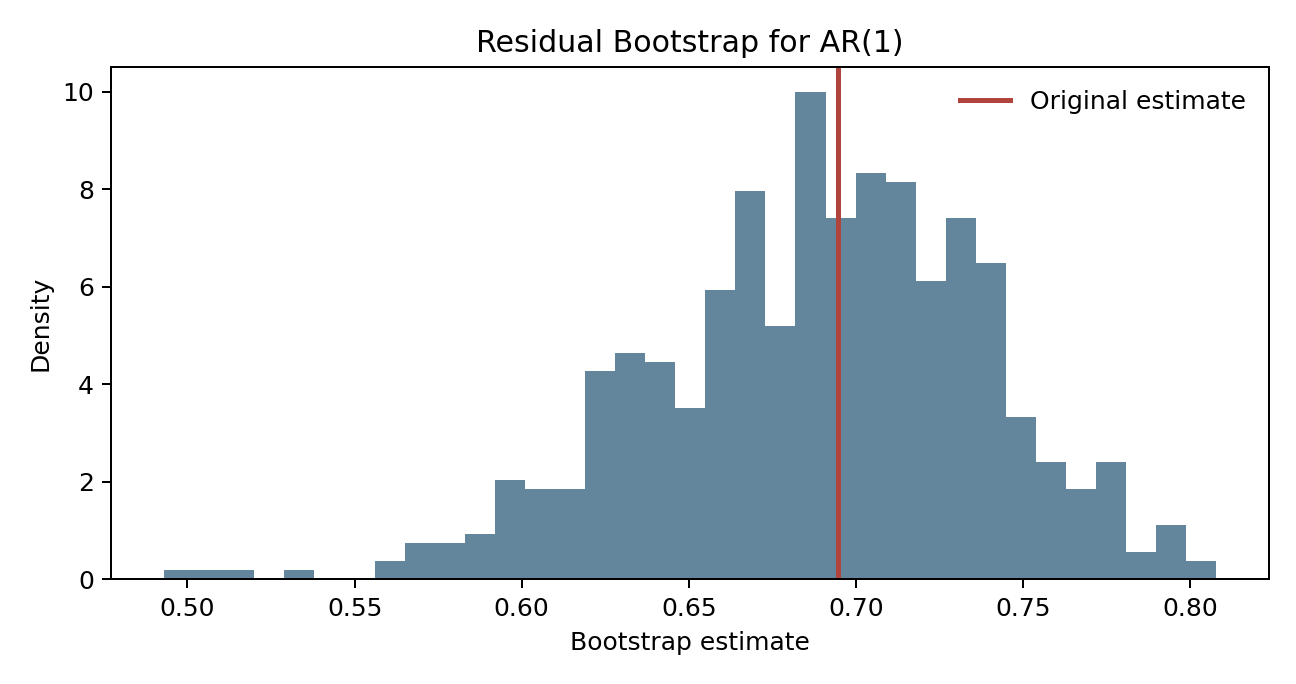
\includegraphics[width=0.86\textwidth]{ch15_fig01_residual_bootstrap.png}
  \caption{AR(1) 残差 Bootstrap 参数分布：重抽样近似估计量的不确定性。}
\end{figure}

\begin{figure}[htbp]
  \centering
  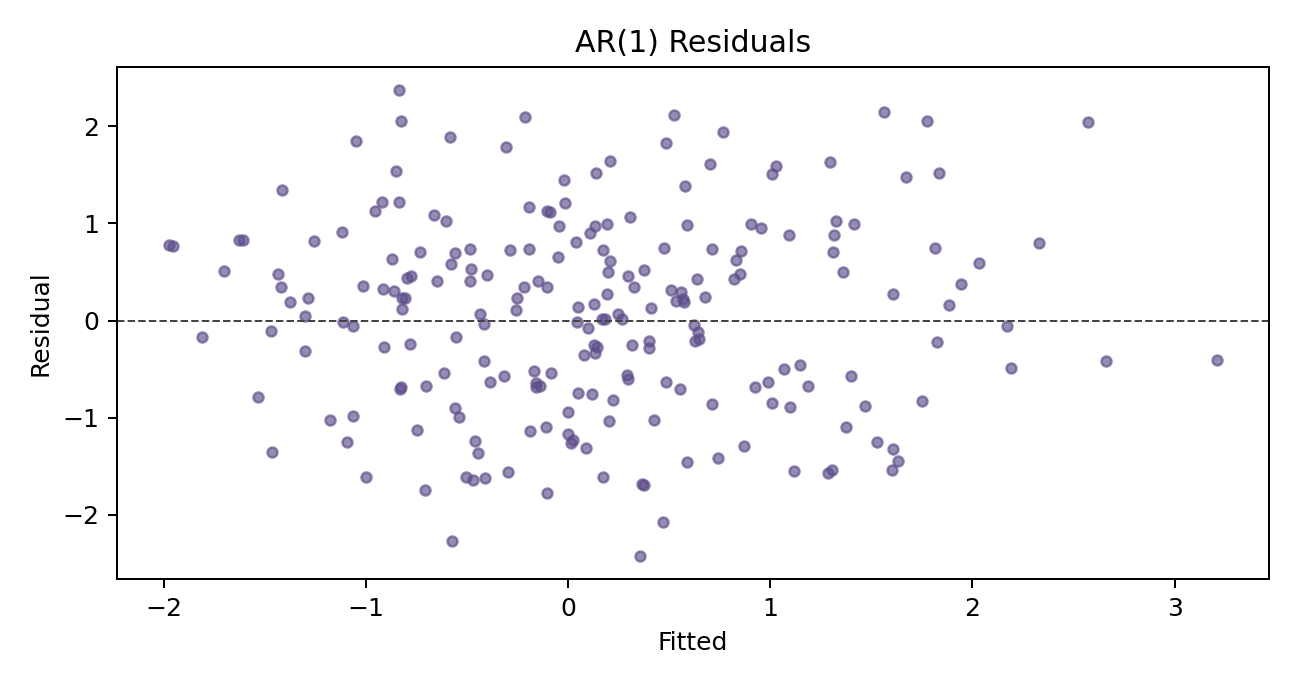
\includegraphics[width=0.86\textwidth]{ch15_fig02_residuals.png}
  \caption{AR(1) 拟合残差图：残差应接近独立同分布创新。}
\end{figure}

\section{练习提要}

原文练习主要围绕下列方向展开：
\begin{itemize}
  \item 手写 AR(1) residual bootstrap 算法；
  \item 比较正态近似区间和 bootstrap 分位数区间；
  \item 研究残差未中心化对 bootstrap 的影响；
  \item 改变 AR 阶数，观察 bootstrap 分布的稳定性。
\end{itemize}

\section*{本章小结}

第 15 章把 bootstrap 引入自回归估计。核心思想是用拟合残差近似未知创新分布，再在拟合模型下重造样本。理论部分说明这种重抽样分布何时能逼近真实估计误差分布。

\end{document}
